\section{Challenge 3 Level 1 (C3L1): Capture The Bug - Given Design (\texttt{riscv\_buggy})}

This challenge involves using the AAPG to create an infrastructure that exposes bugs in the given design. In this section, the methodology or strategy used will be presented, along with its implementation, the results obtained, and finally the conclusion.

\subsection{C3L1: Methodology}

For verifying the Design Under Test (DUT), we have chosen the Functional Verification (FV) methodology. This choice is justified by the existing infrastructure, including the AAPG generation and the comparison method based on the "diff" command between the DUT and the Reference/Golden Model (refmod or spike). Other strategies, such as UVM or Formal Verification, could also be used, but they would require more software and RTL (Register Transfer Level) access.

The fundamental steps of the Functional Verification flow are as follows:

\begin{enumerate}
    \item Study Design;
    \item Define a Verification Plan (VP); 
    \item Implement the test;
    \item Measure, refine and validate (Results);
\end{enumerate}

The process must be repeated if the VP's goals was not reached, otherwise the verification is done. This process is applied to the given design and described in detail in the next Subsections.

\subsection{C3L1: STEP1 - Study Design}

The riscv\_buggy is a black-box RISC-V processor that supports RV32I (RISC-V 32-bit base integer instructions) and CSR (Control and Status Register) instructions (information gotten from Slack). 

Considering this level of knowledge about the system it's appropriate to implement a verification environment to test every instruction specified (RV32I and CSR instructions). The instruction set details are presented in the Annex section \cite{riscv_isa_vol1}. In a real scenario much more should be considered.

The next step is to define a Verification Plan.

\subsection{C3L1: STEP2 - Verification Plan (VP)}

In general, the Verification Plan (VP) is a document that defines the coverage specification, the tests that need to be implemented, and the test architecture.

Based on the information about the DUT, Reference Model (spike), and the AAPG tool, which assists in test creation, the coverage can be based on the expected instructions, and the tests can be designed to leverage the AAPG possibilities. In addition, the traditional verification architecture can be adapted with the available tools. These topics are presented further in the following subsections.

\subsubsection{Coverage Specification}

The verification environment must measure the stimulated instructions and check if all instructions - RV32I and CSR - were covered. It's a stop criterion.

\subsubsection{Test Specification}

In this context, the test specification was divided into 1) sequence generation and 2) test infrastructure (stimulus, comparison, and traceability). 

\paragraph{Sequences generation}

The sequences should be created using AAPG tool. The AAPG allows configuring the group of instructions which is better to understand the bugs. It can be done by configuring the fields in the YAML file. These fields are presented in Listing \ref{lst:c1l3_yaml}. 

\begin{listing}[h!]
\caption{AAPG Configuration.}
\label{lst:c1l3_yaml}
\begin{minted}[frame=single]{nasm}
total_instruction: <config>
rel_sys.csr: <config>
rel_rv32i.ctrl: <config>
rel_rv32i.compute: <config>
rel_rv32i.data: <config>
rel_rv32i.fence: <config>
\end{minted}
\end{listing}

The RV32I instructions can be considered as compute, data, fence, and ctrl. The csr is the Control and Status Register. The field <config> is a value or a weight that the AAPG uses to create the sequences randomly.

An important note is that the ``total\_of\_instructions" field in the first regressions should be kept equal to one or two. This is made to avoid false positives. For example, if a buggy instruction was executed, and its result was saved in register x7, any operation involving x7 could potentially be a false bug. Therefore, by keeping the ``total\_of\_instructions" small and increasing the number of tests, we improve the chances of capturing a real bug. Additionally, each test uses a new seed, which further increases the likelihood of finding a real bug. The planned tests are presented in the next paragraphs.

\paragraph{Test Architecture}

The test architecture is based on the traditional verification architecture, as shown in Figure \ref{fig:arch}. It includes the following steps:

\begin{enumerate}
    \item Stimulus generation represented as ``.bin"
    \item Driving the DUT and the Golden Model.
    \item Comparing the outputs.
    \item Extracting the results (scoreboard).
\end{enumerate}

\begin{figure}[H]
    \centering
    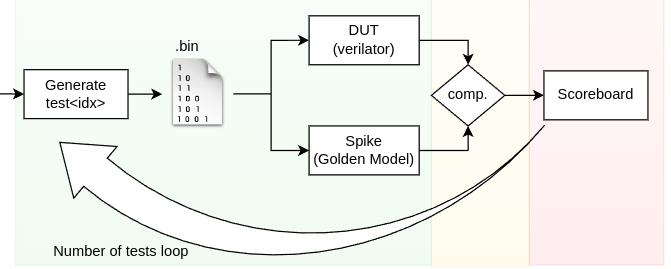
\includegraphics[width=0.5\textwidth]{./c3l1_img/arch.png}
    \caption{Traditional verification architecture adapted to the RISC-V verification environment.}
    \label{fig:arch}
\end{figure}

\subsection{C3L1: STEP1 - Test Implementation}

The sequences planned, and the details about the verification environment implementation are presented in this Section.

\subsubsection{Sequences}

The sequences were planned to separate the group of analysis due to the facilitate associate in analysis and debugging.

\paragraph{TEST\_ONLY\_DATA}

The configuration file is presented in Listing \ref{lst:c1l3_tod}. It will generate only data instructions (lw, sw, li, sh, lh, etc).

\begin{listing}[h!]
\caption{TEST\_ONLY\_DATA.}
\label{lst:c1l3_tod}
\begin{minted}[frame=single]{nasm}
  rel_sys.csr: 0
  rel_rv32i.ctrl: 0
  rel_rv32i.compute: 0
  rel_rv32i.data: 1
  rel_rv32i.fence: 0
\end{minted}
\end{listing}

\paragraph{TEST\_ONLY\_COMPUTE}

The configuration file is presented in Listing \ref{lst:c1l3_toc}. It will generate only compute instructions (or, xor, add, addi, sub, etc).

\begin{listing}[h]
\caption{TEST\_ONLY\_COMPUTE.}
\label{lst:c1l3_toc}
\begin{minted}[frame=single]{nasm}
  rel_sys.csr: 0
  rel_rv32i.ctrl: 0
  rel_rv32i.compute: 1
  rel_rv32i.data: 0
  rel_rv32i.fence: 0
\end{minted}
\end{listing}

\paragraph{TEST\_CSR\_DATA\_FENCE}

The configuration file is presented in Listing \ref{lst:c1l3_tcdf}. It will generate data, fence, and csr instructions. In this case, it's not possible to isolate CSR, then data and fence were set to allow the generation.s

In addition, the total instruction needs to be increased to fit the distribution specification.

\begin{listing}[ht]
\caption{TEST\_CSR\_DATA\_FENCE.}
\label{lst:c1l3_tcdf}
\begin{minted}[frame=single]{nasm}
    total_instructions: 3 # needed
    rel_sys.csr: 1 # focus
    rel_rv32i.ctrl: 0
    rel_rv32i.compute: 0 
    rel_rv32i.data: .5
    rel_rv32i.fence: .5
\end{minted}
\end{listing}

\paragraph{TEST\_CTRL\_DATA}

The configuration file is presented in Listing \ref{lst:c1l3}. It will generate Ctrl (control) and data instructions. Also, it's not possible to isolate Ctrl, then data was included in the generation.

In addition, the total instruction needs to be increased to fit the distribution specification.

\begin{listing}[h!]
\caption{TEST\_CTRL\_DATA.}
\label{lst:c1l3}
\begin{minted}[frame=single]{nasm}
    total_instructions: 500
    rel_sys.csr: 0 
    rel_rv32i.ctrl: 0.2 # focus
    rel_rv32i.compute: 0 
    rel_rv32i.data: 2
    rel_rv32i.fence: 0
    \end{minted}
\end{listing}

\subsubsection{Test Implementation}

The test infrastructure was implemented in Python (file: \texttt{run\_tests.py}) in three steps, as shown in Figure \ref{fig:implement}.

\begin{figure*} % Use figure* to make the figure span the whole page
    \centering
    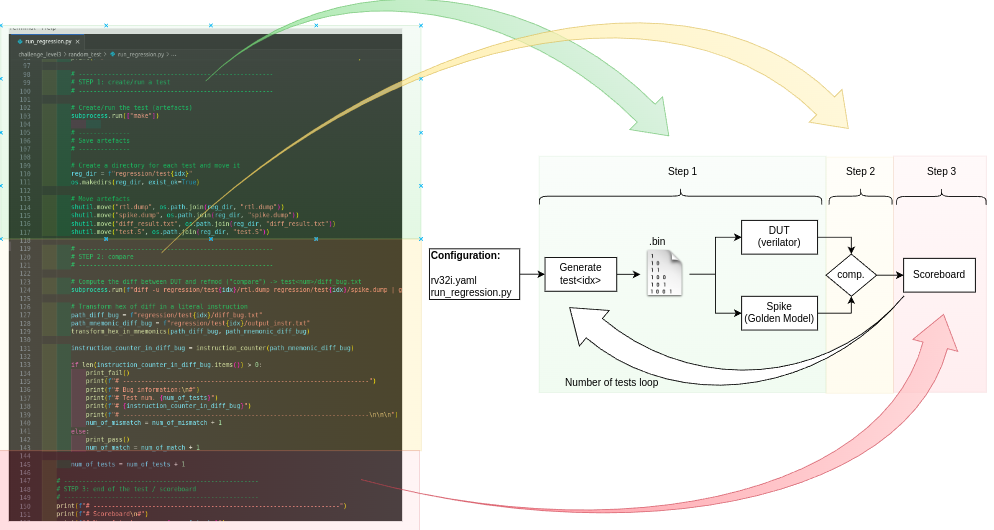
\includegraphics[width=1\textwidth]{./c3l1_img/implement.png} % This sets the image width to the text width
    \caption{Steps for the test implementation.}
    \label{fig:implement}
\end{figure*}

The routines are based on these three steps. Step 1 calls the Makefile (\# make) and performs the following actions: AAPG generation, cross-compilation of the generated test.S using the RISC-V Toolchain, stimulation (spike and verilator dut), and comparison of the models' outputs using the ``diff" command. Step 2 reads the generated ``diff" file, verifies if it is empty or not, and increments the ``match" variable with a PASS message if it is empty, or increments the ``mismatch" variable and presents information about the bug (see Figure \ref{fig:fail}). Finally, Step 3 prints the scoreboard as shown in Figure \ref{fig:scb}. 

Before executing this script, the test configuration (TEST\_ONLY\_DATA, TEST\_ONLY\_COMPUTE, etc.) and the number of tests (set by the variable ``num\_of\_tests" inside \texttt{run\_tests.py}) must be defined. After that, the script can be run (\# python3 \texttt{run\_tests.py}). The main infrastructure is based on the last challenges learned.

\begin{figure}[H]
    \centering
    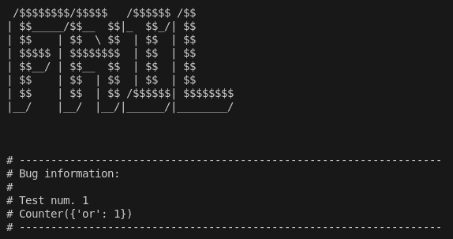
\includegraphics[width=0.47\textwidth]{./c3l1_img/fail.png}
    \caption{Bug information presentation.}
    \label{fig:fail}
\end{figure}

\begin{figure}[H]
    \centering
    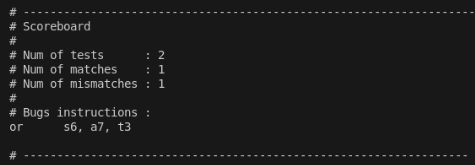
\includegraphics[width=0.48\textwidth]{./c3l1_img/scb.png}
    \caption{Scoreboard presentation.}
    \label{fig:scb}
\end{figure}

Another script (\texttt{run\_analysis\_reg.py}) was implemented for generating histograms and conducting coverage analysis. After executing regressions (see Figure \ref{fig:regressions_sample}), this script reads the generated artifacts, calculates the number of executed instructions and their percentage, plots the histogram, and calculates the percentage of instructions exercised compared to all expected instructions (Annex). In summary, it implements the coverage analysis by reading the dump files, applying disassembly, and measuring the instructions from that.

\begin{figure}[H]
    \centering
    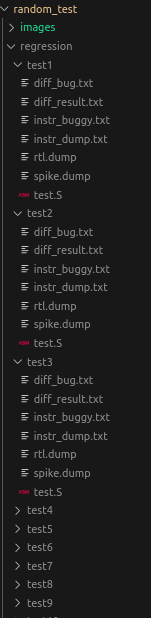
\includegraphics[width=0.19\textwidth]{./c3l1_img/regressions_sample.png}
    \caption{Sample of regressions execution.}
    \label{fig:regressions_sample}
\end{figure}

The results obtained from applying the defined Methodology will be presented in this section, along with the bugs found. 

\subsection{C3L1 Results: TEST\_ONLY\_DATA - Regression 1}

\subsubsection{Configuration}

\begin{itemize}
    \item num\_of\_tests = 10
    \item total\_instructions = 2
\end{itemize}

\subsubsection{Result}
PASS.

\begin{figure}[H]
    \centering
    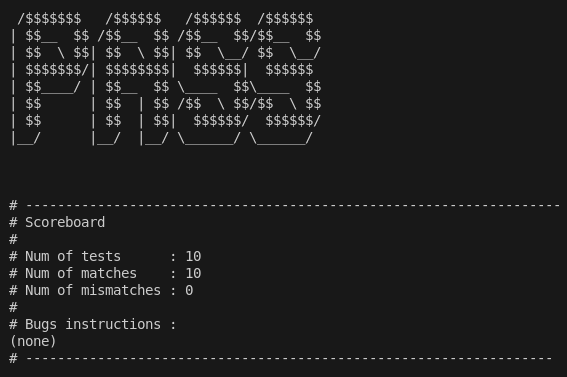
\includegraphics[width=0.47\textwidth]{./c3l1_img/tod_10_r.png}
    \caption{Regression 1 results for TEST\_ONLY\_DATA.}
    \label{fig:tod\_10\_r}
\end{figure}

\subsubsection{Histogram of instructions stimulated}

Even configuring only data, the initialization of the system uses other instructions, then this is captured in the analysis.

\subsection{C3L1 Results: TEST\_ONLY\_DATA - Regression 2}


\subsubsection{Configuration}
\begin{itemize}
    \item num\_of\_tests = 100
    \item total\_instructions = 20
\end{itemize}

\subsubsection{Result}
PASS.

\begin{figure}[H]
    \centering
    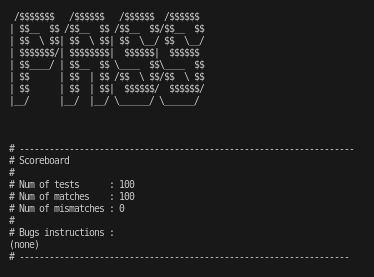
\includegraphics[width=0.53\textwidth]{./c3l1_img/tod_100_r.png}
    \caption{Regression 2 results for TEST\_ONLY\_DATA.}
    \label{fig:tod_100_r}
\end{figure}

\subsubsection{Histogram of instructions stimulated}

The instructions kept the same but the frequency increased compared to regression 1 (see Figure \ref{fig:tod_10}
 and \ref{fig:tod_100}.
 
\begin{figure}[ht]
    \centering
    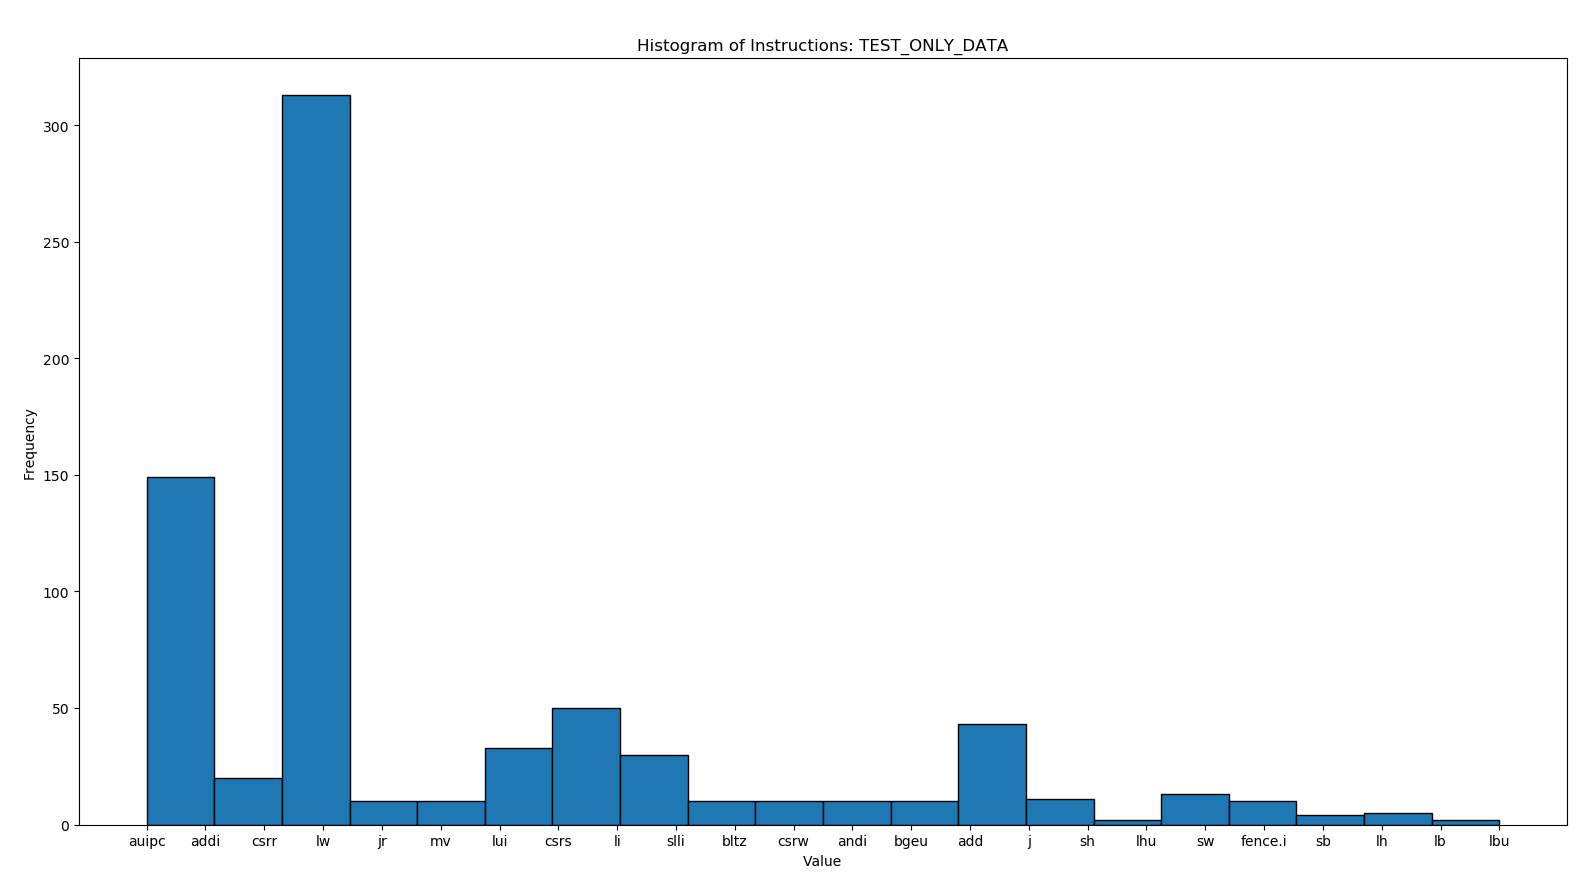
\includegraphics[width=0.48\textwidth]{./c3l1_img/tod_10.png}
    \caption{Histogram of instructions stimulated for TEST\_ONLY\_DATA (regression 1).}
    \label{fig:tod_10}
\end{figure}


\subsubsection{Discussion and Coverage Status}

Two regressions were executed. The first one with 10 tests and 2 instructions, but no bugs were encountered. The second regression, with 100 tests and 20 instructions, still did not find any bugs. It suggests that the bug might not be in the RV32I.data set (see the histogram).

The coverage was calculated for this case and, as expected, it did not reach 100\% since it is a subset of all instructions.

\begin{figure}[H]
    \centering
    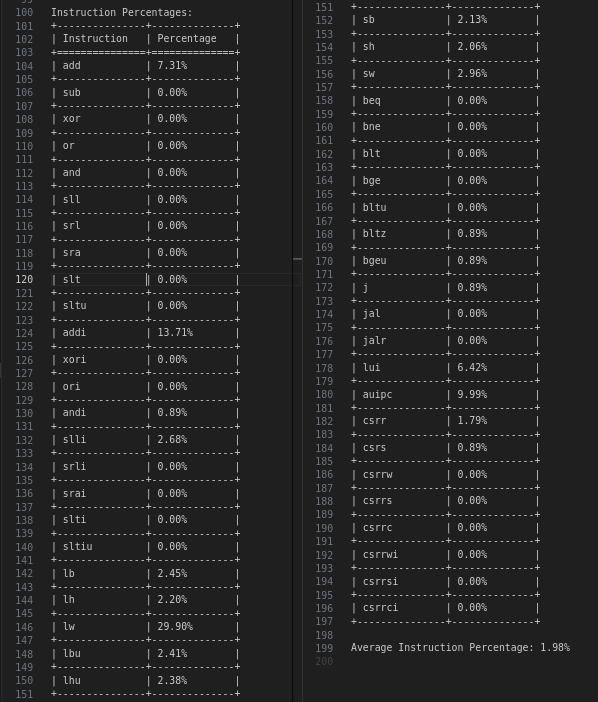
\includegraphics[width=0.48\textwidth]{./c3l1_img/cov_t0.png}
    \caption{Coverage for TEST\_ONLY\_DATA.}
    \label{fig:cov_t0}
\end{figure}

\begin{verbatim}
Instructions Tested: 24/47
Percentage Instructions Tested: 51.06%
\end{verbatim}

\begin{figure}[H]
    \centering
    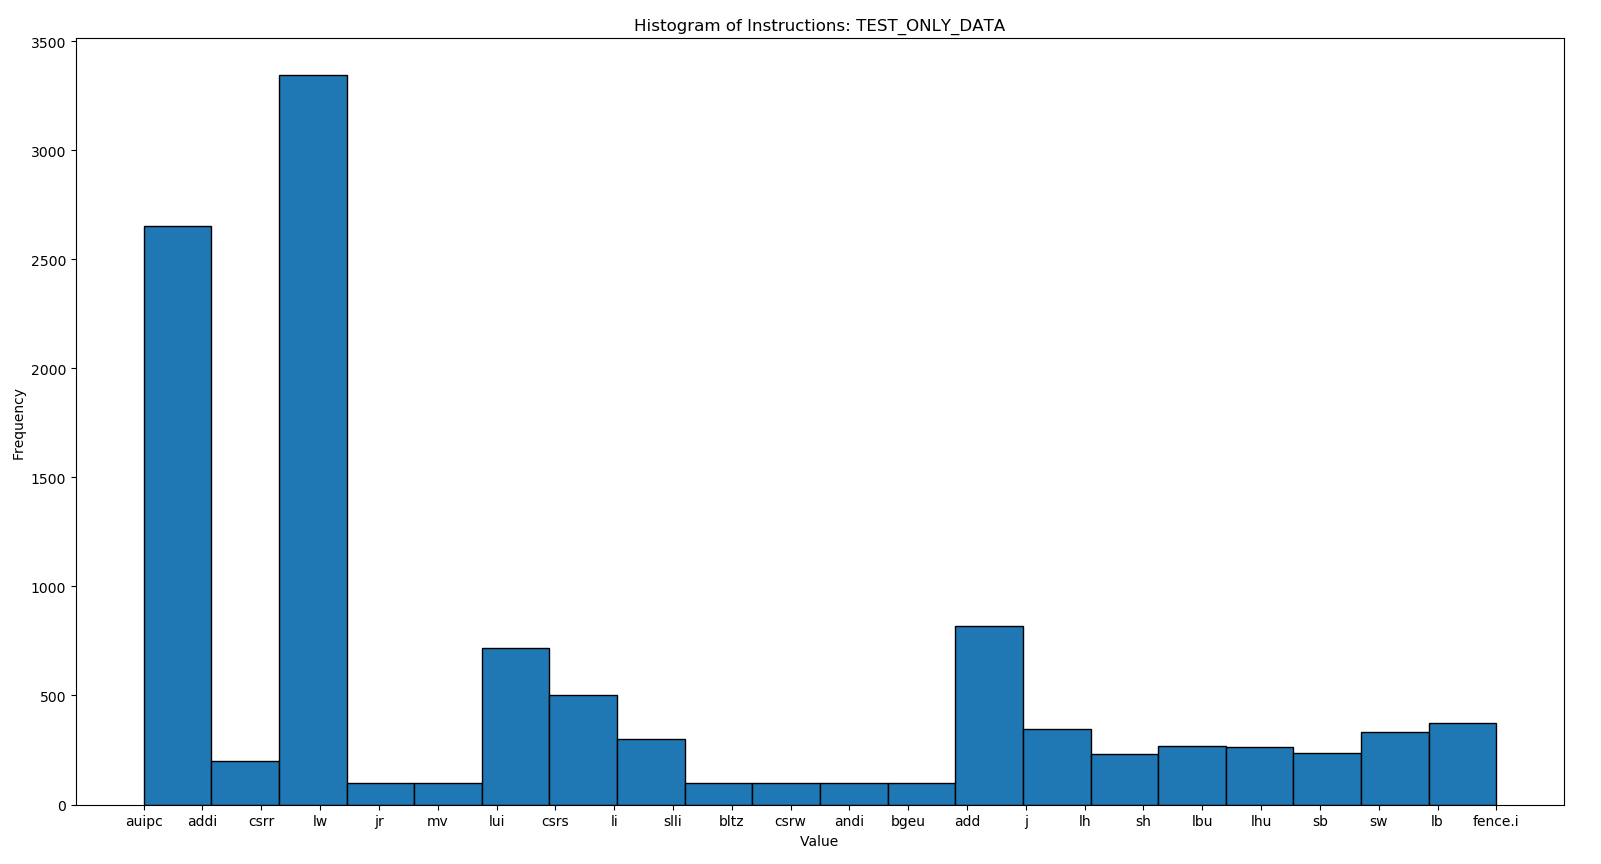
\includegraphics[width=0.5\textwidth]{./c3l1_img/tod_100.png}
    \caption{Histogram of instructions stimulated for TEST\_ONLY\_DATA (regression 2).}
    \label{fig:tod_100}
\end{figure}

\subsection{C3L1 Results: TEST\_ONLY\_COMPUTE-Regression1}

\subsubsection{Configuration}

\begin{itemize}
    \item num\_of\_tests = 10
    \item total\_instructions = 2
\end{itemize}

\subsubsection{Result}
The scoreboard captured bugs in the instructions compute OR and ORI. An deep investigation is presented after regressions.

\begin{figure}[H]
    \centering
    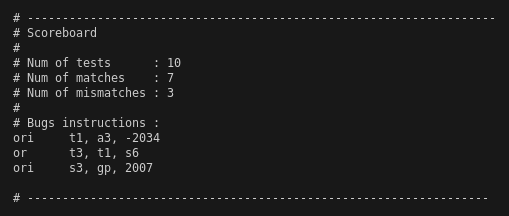
\includegraphics[width=0.5\textwidth]{./c3l1_img/toc_10_r.png}
    \caption{Regression 1 results for TEST\_ONLY\_COMPUTE.}
    \label{fig:toc_10_r}
\end{figure}

\subsubsection{Histogram of instructions stimulated}
as expected the compute instructions are presented.

\begin{figure}[H]
    \centering
    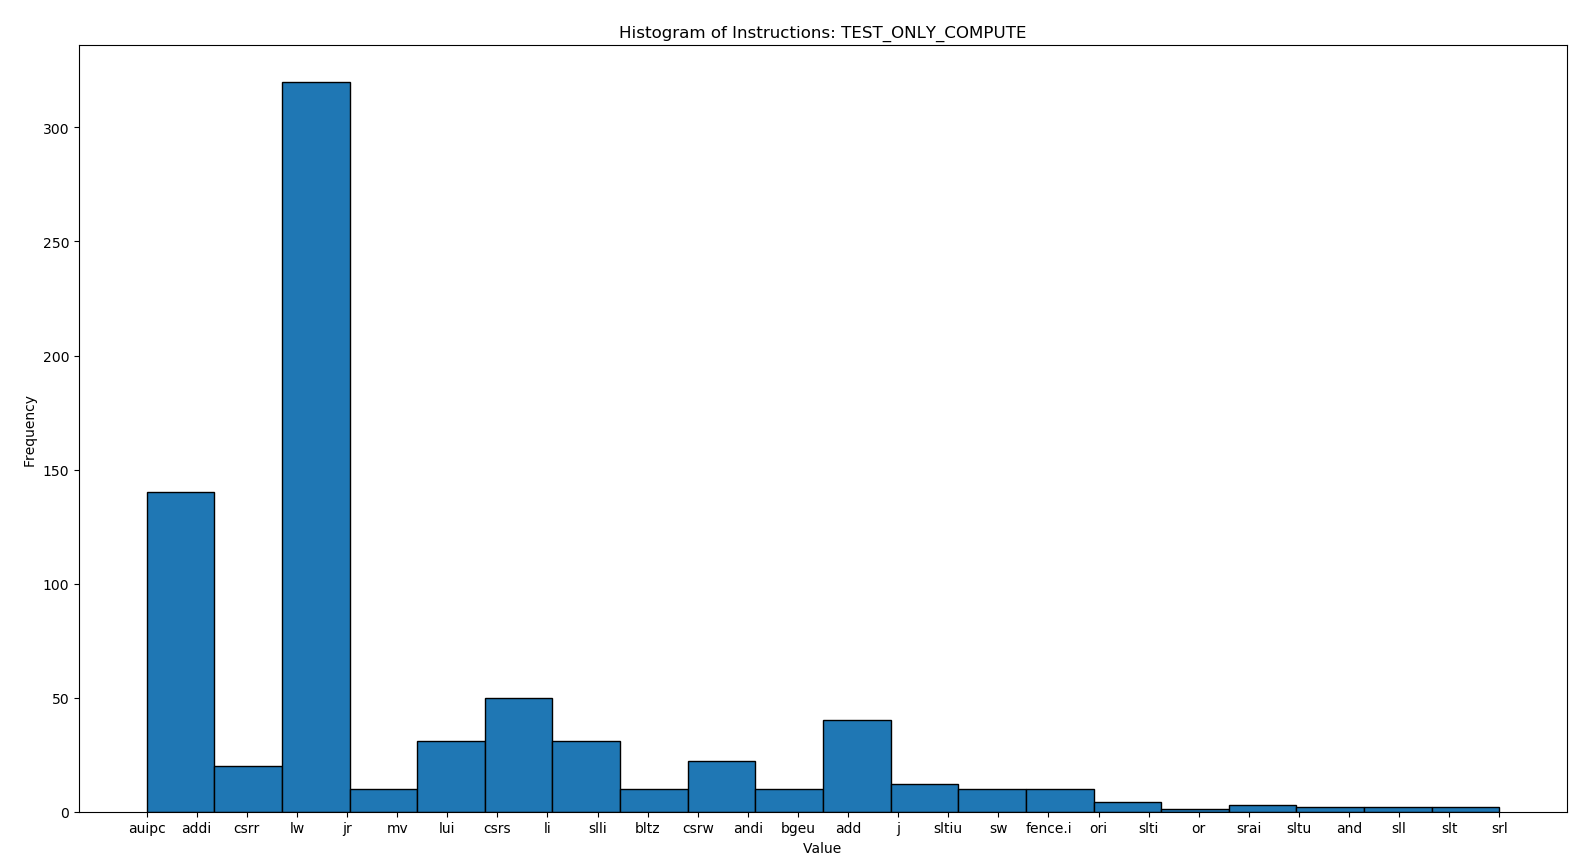
\includegraphics[width=0.48\textwidth]{./c3l1_img/toc_10.png}
    \caption{Histogram of instructions stimulated for TEST\_ONLY\_COMPUTE.}
    \label{fig:toc_10}
\end{figure}

\subsection{C3L1 Results: TEST\_ONLY\_COMPUTE-Regression2}

\subsubsection{Configuration}

\begin{itemize}
    \item num\_of\_tests = 100
    \item total\_instructions = 2
\end{itemize}

\subsubsection{Result}
Scoreboard.

\begin{figure}[H]
    \centering
    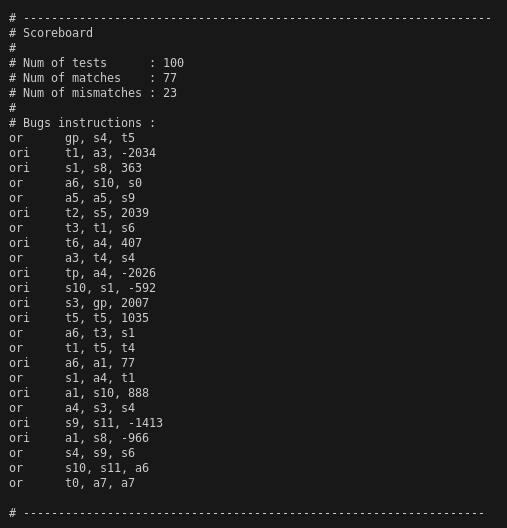
\includegraphics[width=0.47\textwidth]{./c3l1_img/toc_100_r.png}
    \caption{Regression 2 results for TEST\_ONLY\_COMPUTE.}
    \label{fig:toc_100_r}
\end{figure}

\subsubsection{Histogram of instructions stimulated}
as expected the compute instructions are presented.


\begin{figure}[H]
    \centering
    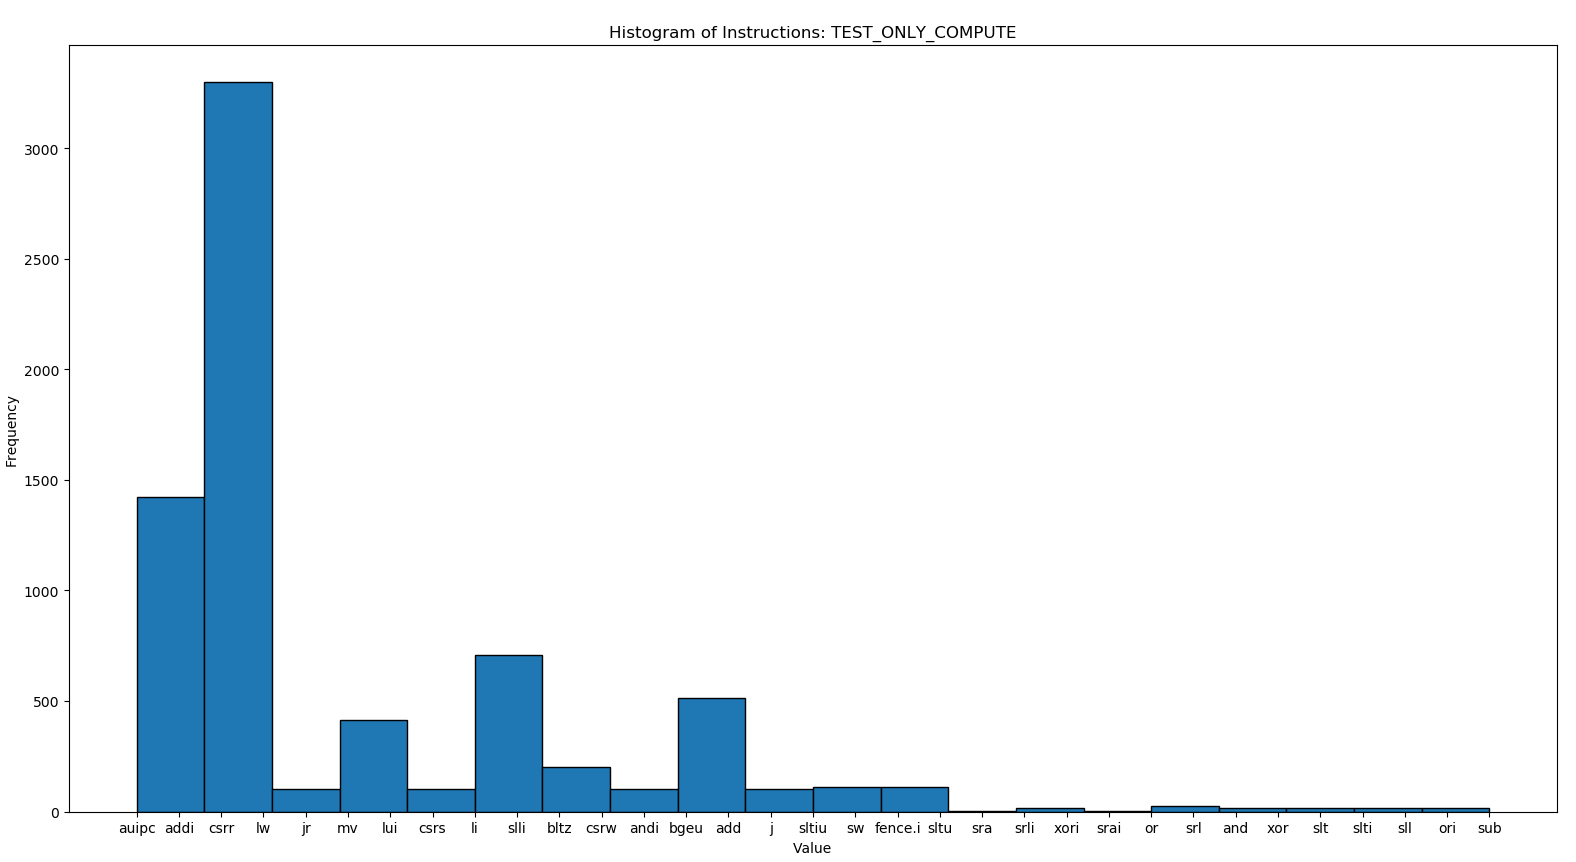
\includegraphics[width=0.5\textwidth]{./c3l1_img/toc_100.png}
    \caption{Histogram of instructions stimulated for TEST\_ONLY\_COMPUTE.}
    \label{fig:toc_100}
\end{figure}

\subsubsection{Discussion and Coverage Status}

The test captured a bug in the OR and ORI instruction. To understand the cause of the bug, let's consider the scenario presented below.

\begin{figure*}
    \centering
    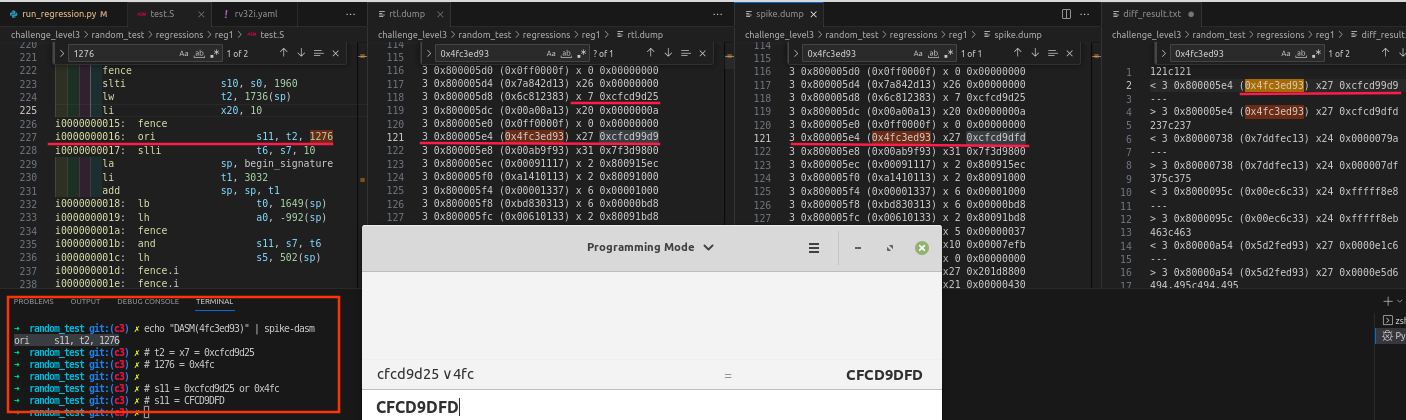
\includegraphics[width=1\textwidth]{./c3l1_img/ori_bug_anal2.png}
    \caption{Analysis of the ORI bug.}
    \label{fig:ori_bug_anal2}
\end{figure*}

By analyzing the literal operation (Figure \ref{fig:ori_bug_anal}), it's possible to understand the real cause of the bug. When A and B are equal to 1, the output bit expected is inverted. The OR instruction also has a similar bug, and the same analysis can be done to verify the cause in detail.

\begin{figure}[H]
    \centering
    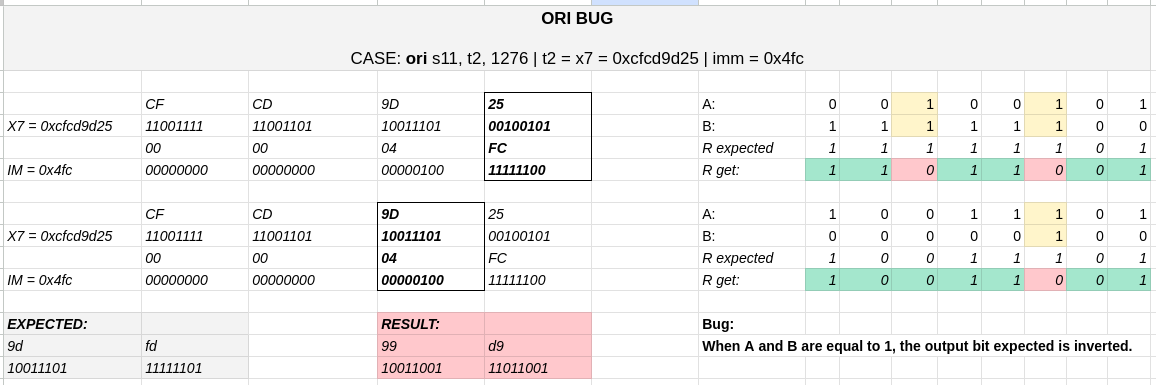
\includegraphics[width=0.5\textwidth]{./c3l1_img/ori_bug_anal.png}
    \caption{Analysis of the ORI bug.}
    \label{fig:ori_bug_anal}
\end{figure}

\textbf{Important note: }Increasing the number of instructions in this test will return many bugs. However, without accurate analysis, it's hard to identify if it is a real bug or generated due to the wrong value assigned to registers after the OR or ORI operation creating a false positive (or "fake" bug). Therefore, it's safer and easier, in terms of bug capture, to keep the number of instructions equal to one or two and increase the number of tests.

\subsubsection{Coverage}

The coverage was calculated in regression 2, and the result is shown below. The increase in coverage is due to the set of instructions configured. The compute set (add, xor, xori, etc.) is greater than the compute data set. As a result, the coverage reached 70.21\%.

\begin{verbatim}
Instructions Tested: 33/47
Percentage Instructions Tested: 70.21%
\end{verbatim}

\subsection{C3L1 Results: TEST\_CSR\_DATA\_FENCE - Regr. 1}

\subsubsection{Configuration}

\begin{itemize}
    \item num\_of\_tests = 30
    \item total\_instructions = 3
\end{itemize}

\subsubsection{Result}

No bugs were encountered in this case.

\subsection{C3L1 Results: TEST\_CSR\_DATA\_FENCE - Regr. 2}

\subsubsection{Configuration}

\begin{itemize}
    \item num\_of\_tests = 30
    \item total\_instructions = 10
\end{itemize}

\subsubsection{Result}
The instruction \textbf{csrrci} appears in the Spike dump but not in the RTL dump due to this inconsistency the test environment returns a bug as presented in Figure \ref{fig:tcdf_reg2}). However, apparently the bug is related to the tool and not to the design. As a result, it will be not considered a bug in riscv\_buggy.

\begin{figure}[H]
    \centering
    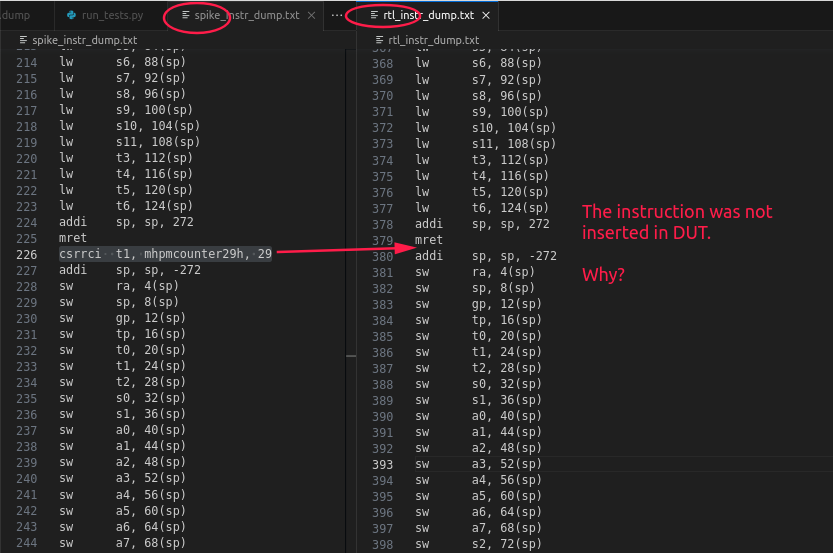
\includegraphics[width=0.5\textwidth]{./c3l1_img/tcdf_reg2.png}
    \caption{Regression 2 results for TEST\_CSR\_DATA\_FENCE.}
    \label{fig:tcdf_reg2}
\end{figure}

\subsection{C3L1 Results: TEST\_CTRL\_DATA}

The method was executed under this configuration, and it demonstrated exceptional stability with no encountered bugs, even during exhaustive stimulation.

\subsection{C3L1: Conclusion riscv\_buggy}

Based on the tested extensions and strategy, the result of riscv\_buggy verification is summarized below. In other words, the tests encountered bugs in the OR and ORI instructions and a inconsistency in CSR.

\begin{verbatim}
# Extension        # RESULT/STATUS
rel_sys.csr        # INCONSISTENT
rel_rv32i.ctrl:    # NO BUGS
rel_rv32i.compute: # BUGS: OR/ORI instr.
rel_rv32i.data:    # NO BUGS
rel_rv32i.fence:   # NO BUGS
\end{verbatim}

Considering all the regression results, the specified coverage reaches 100\%. However, it is important to note that due to the encountered bugs, merging the results might not provide a meaningful representation of the overall coverage in this case. The identified bugs should be carefully addressed and resolved before concluding the final coverage assessment.

In a real development flow, these results should be discussed with the designer responsible to address the problems. After that, the same tests should pass, and finally, a refinement in the VP also should be made to stimulate in different ways the design and achieve coverage.